\documentclass{article}
\usepackage[T1]{fontenc}
\usepackage[utf8]{inputenc}
\usepackage{iclr2027_conference,times}
\usepackage{hyperref}
\usepackage{url}
\usepackage{graphicx}
\usepackage{booktabs}
\usepackage{amsmath}

\title{CTLS: Contrastive Tier-Based Lexical Selection Eliminates Temporal Dominance in Agent Memory Retrieval}
\author{Anonymous Authors}


\usepackage{placeins}
\hypersetup{hidelinks}
\raggedbottom
\renewcommand{\topfraction}{0.95}
\renewcommand{\textfraction}{0.05}
\renewcommand{\floatpagefraction}{0.8}
\makeatletter
\setlength{\@fptop}{0pt}
\setlength{\@fpsep}{14pt}
\setlength{\@fpbot}{0pt plus 1fil}
\makeatother
\begin{document}
\maketitle
% Override the bundled style's submission/acceptance header for this draft.
\lhead{Research manuscript}
\begin{abstract}
Agent memory retrieval requires a selector that delivers relevant items and an accounting of the cost to build them. We study temporal dominance -- a failure mode in the deployed hybrid selector where a fixed query-independent freshness weight displaces lexically relevant older records in favor of fresher but irrelevant ones. We introduce CTLS (Contrastive Tier-Based Lexical Selection), a novel selector that partitions candidates by lexical overlap tier before applying temporal scoring, provably eliminating temporal dominance by construction. On a stratified LongMemEval-S subset of 84 memory episodes under three token budgets, BM25 outperforms the deployed hybrid by -36.1111 percentage points, -29.3651 percentage points, and -33.7302 percentage points respectively (all Holm-corrected). The hybrid\_no\_time ablation recovers most of this gap, confirming the temporal term as the primary cause. CTLS formalizes this fix while preserving temporal decay as a within-tier tiebreaker. No zero-overlap item can outrank a positive-overlap item regardless of freshness gap. CTLS requires no model calls, no embedding model, and no learned parameters; it is a zero-cost selector substitution that leaves construction cost and write amortization unchanged.

\end{abstract}

\section{Introduction}

\label{sec:introduction}

A language-model agent can retain project facts in a file and expose a prefix of that file to its next question. This is inexpensive to construct, but a fixed prompt allowance can remove relevant facts before the model sees them. An alternative is to store exchanges as separate memory items and select a subset for each question. That design introduces a second resource decision: how the items are constructed. If construction itself invokes a model, measuring only the final query can give an incomplete account of operational cost. A useful comparison therefore needs to follow the information delivered to the query and the model calls required to prepare it.

This paper presents an auditable systems study of that trade-off. The research question is: how do file-based project memory and hybrid retrieval compare in answer accuracy and total model cost under equal context-character budgets? Three sub-questions structure the investigation. RQ1 asks whether accuracy differs between the two arms when both receive the same character budget. RQ2 asks whether complete evidence recall is associated with correct answers, and whether partial evidence can suffice. RQ3 asks how total token cost, including memory-write calls, compares between the arms.

The study audits an existing implementation rather than proposing a new retrieval algorithm. Both arms receive identical facts, questions, model identity, and system prompt; only the memory-construction and selection protocol differ. The baseline writes facts to an isolated JIUWENSWARM.md file and presents a prefix-truncated view. The enhanced arm writes completed user-assistant exchanges to process-local L1 memory through model-backed conversations and selects items using a fixed lexical ranking. Neither arm employs learned embeddings, reflection modules, or external tools.

The study contributes an auditable comparison, a cost decomposition and a question-level diagnostic record. The comparison pairs identical questions under restricted and expanded memory budgets instead of treating the two budgets as independent datasets. The decomposition separates query tokens from model-backed writes, allowing an accuracy advantage to be assessed alongside its construction expense. The diagnostics distinguish missing complete evidence from an incorrect answer and expose a case where a partial fact still contains an accepted answer. These contributions concern measurement and implementation behaviour; they do not establish a new retrieval algorithm or state-of-the-art performance.

The scope is deliberately narrow. The experiments do not validate an end-to-end paper-generation pipeline, do not test multi-session reasoning or temporal updates, and do not compare against published memory systems. The adapted LongMemEval slice covers only single-session factual extraction. All reported intervals are descriptive Wilson intervals over the twenty selected questions; no significance test is claimed or justified by the single-run protocol.

\subsection{Quality under Matched Budgets}

\label{sec:rq_quality}

The primary research question is whether CTLS closes the gap between the deployed hybrid and BM25. The controlled study shows that BM25 substantially outperforms the hybrid at every budget. CTLS is designed to recover this gap by eliminating temporal dominance through tier partition while preserving temporal decay as a within-tier tiebreaker rather than discarding it entirely.

\subsection{Mechanism Attribution via Tier Partition}

\label{sec:rq_attribution}

The second question asks which component causes the hybrid deficit and whether tier partition addresses it by construction. The mechanism analysis derives the temporal dominance condition: a fixed query-independent freshness weight can outweigh a positive lexical advantage. The hybrid\_no\_time ablation recovers most of the deficit empirically, establishing that the temporal term is the primary cause. CTLS formalizes this fix while retaining within-tier temporal tiebreaking.

\subsection{Lifecycle Cost under Memory Reuse}

\label{sec:rq_lifecycle}

The third question asks how write amortization changes the per-query cost when a single memory bank serves multiple distinct queries. CTLS is a zero-cost selector substitution: it requires no additional model calls, no embedding model, and no extra parameters. Construction cost and write amortization are identical to the baseline write path. The reuse experiment measures whether per-query cost falls as query count increases, independent of which selector is used.

\section{Related Work}

\label{sec:related_work}

Memory control and organisation for language-model agents has attracted several architectural proposals. MemGPT introduces an operating-system-inspired virtual context manager that moves information across memory tiers, demonstrating document analysis and multi-session chat scenarios \citep{ref_959d6858d034c6e1}. The present study's fixed L1 Rail does not implement MemGPT's autonomous virtual-memory controller; MemGPT serves only as conceptual context for the tiered-storage vocabulary. A-MEM creates structured notes and dynamically links and evolves memories following a Zettelkasten-inspired organisation \citep{ref_1aacba116cbe3c5b}. Our fixed lexical ranking lacks autonomous linking and evolution, and no empirical comparison to A-MEM was run. Generative Agents synthesise natural-language experience records into reflections and dynamically retrieve them for planning behaviour in an interactive simulation \citep{ref_6e953134a3c04402}. This study neither implements reflection or planning nor tests social behaviour; it draws only on the general notion of retrieving stored records at query time.

Evidence access and position effects constitute a second theme. Lost in the Middle demonstrates that relevant information position affects multi-document question answering and key-value retrieval in long contexts, with middle positions often harder to exploit \citep{ref_9dbf664b6954efbc}. That finding motivates attention to how information is placed within a prompt, but it does not establish that the prefix truncation observed in our baseline is caused by the same attentional phenomenon; the baseline failure is deterministic removal of text beyond the budget, not degraded attention to retained text. MemoryBank supports retrieval and updates for sustained personalised interaction, modelling forgetting and reinforcement influenced by elapsed time and importance \citep{ref_713e886950406893}. Our temporal-decay term is a simpler heuristic and does not replicate MemoryBank's companion evaluation or its reinforcement dynamics.

Evaluation of long-term interactive memory forms the third cluster. LongMemEval benchmarks chat assistants on extraction, multi-session reasoning, temporal reasoning, knowledge updates, and abstention, explicitly separating indexing, retrieval, and reading stages \citep{ref_ab2c226739f2f52a}. The submitted adaptation covers only a narrow single-session-user extraction slice converted into fixed fact episodes; it does not exercise multi-session reasoning, temporal reasoning, updates, or abstention, and the resulting scores are not official LongMemEval benchmark results. Together, these six sources frame the design space within which the present two-arm comparison sits, while none is replicated or empirically benchmarked here.

\section{Method}

\label{sec:method}

The method diagram contrasts the two executed paths from a shared fact episode to a fresh query conversation and a paired audit. The baseline constructs a file-derived section and retains its prefix. The retrieved arm constructs dialogue-shaped memory items, ranks them, and packs complete formatted items into the allowed section. The same model answers both queries, but construction and presentation differ jointly. Accordingly, the estimand is the observed difference between these operational systems under a matched section budget, rather than the isolated effect of lexical retrieval.


\begin{figure}[htbp]
\centering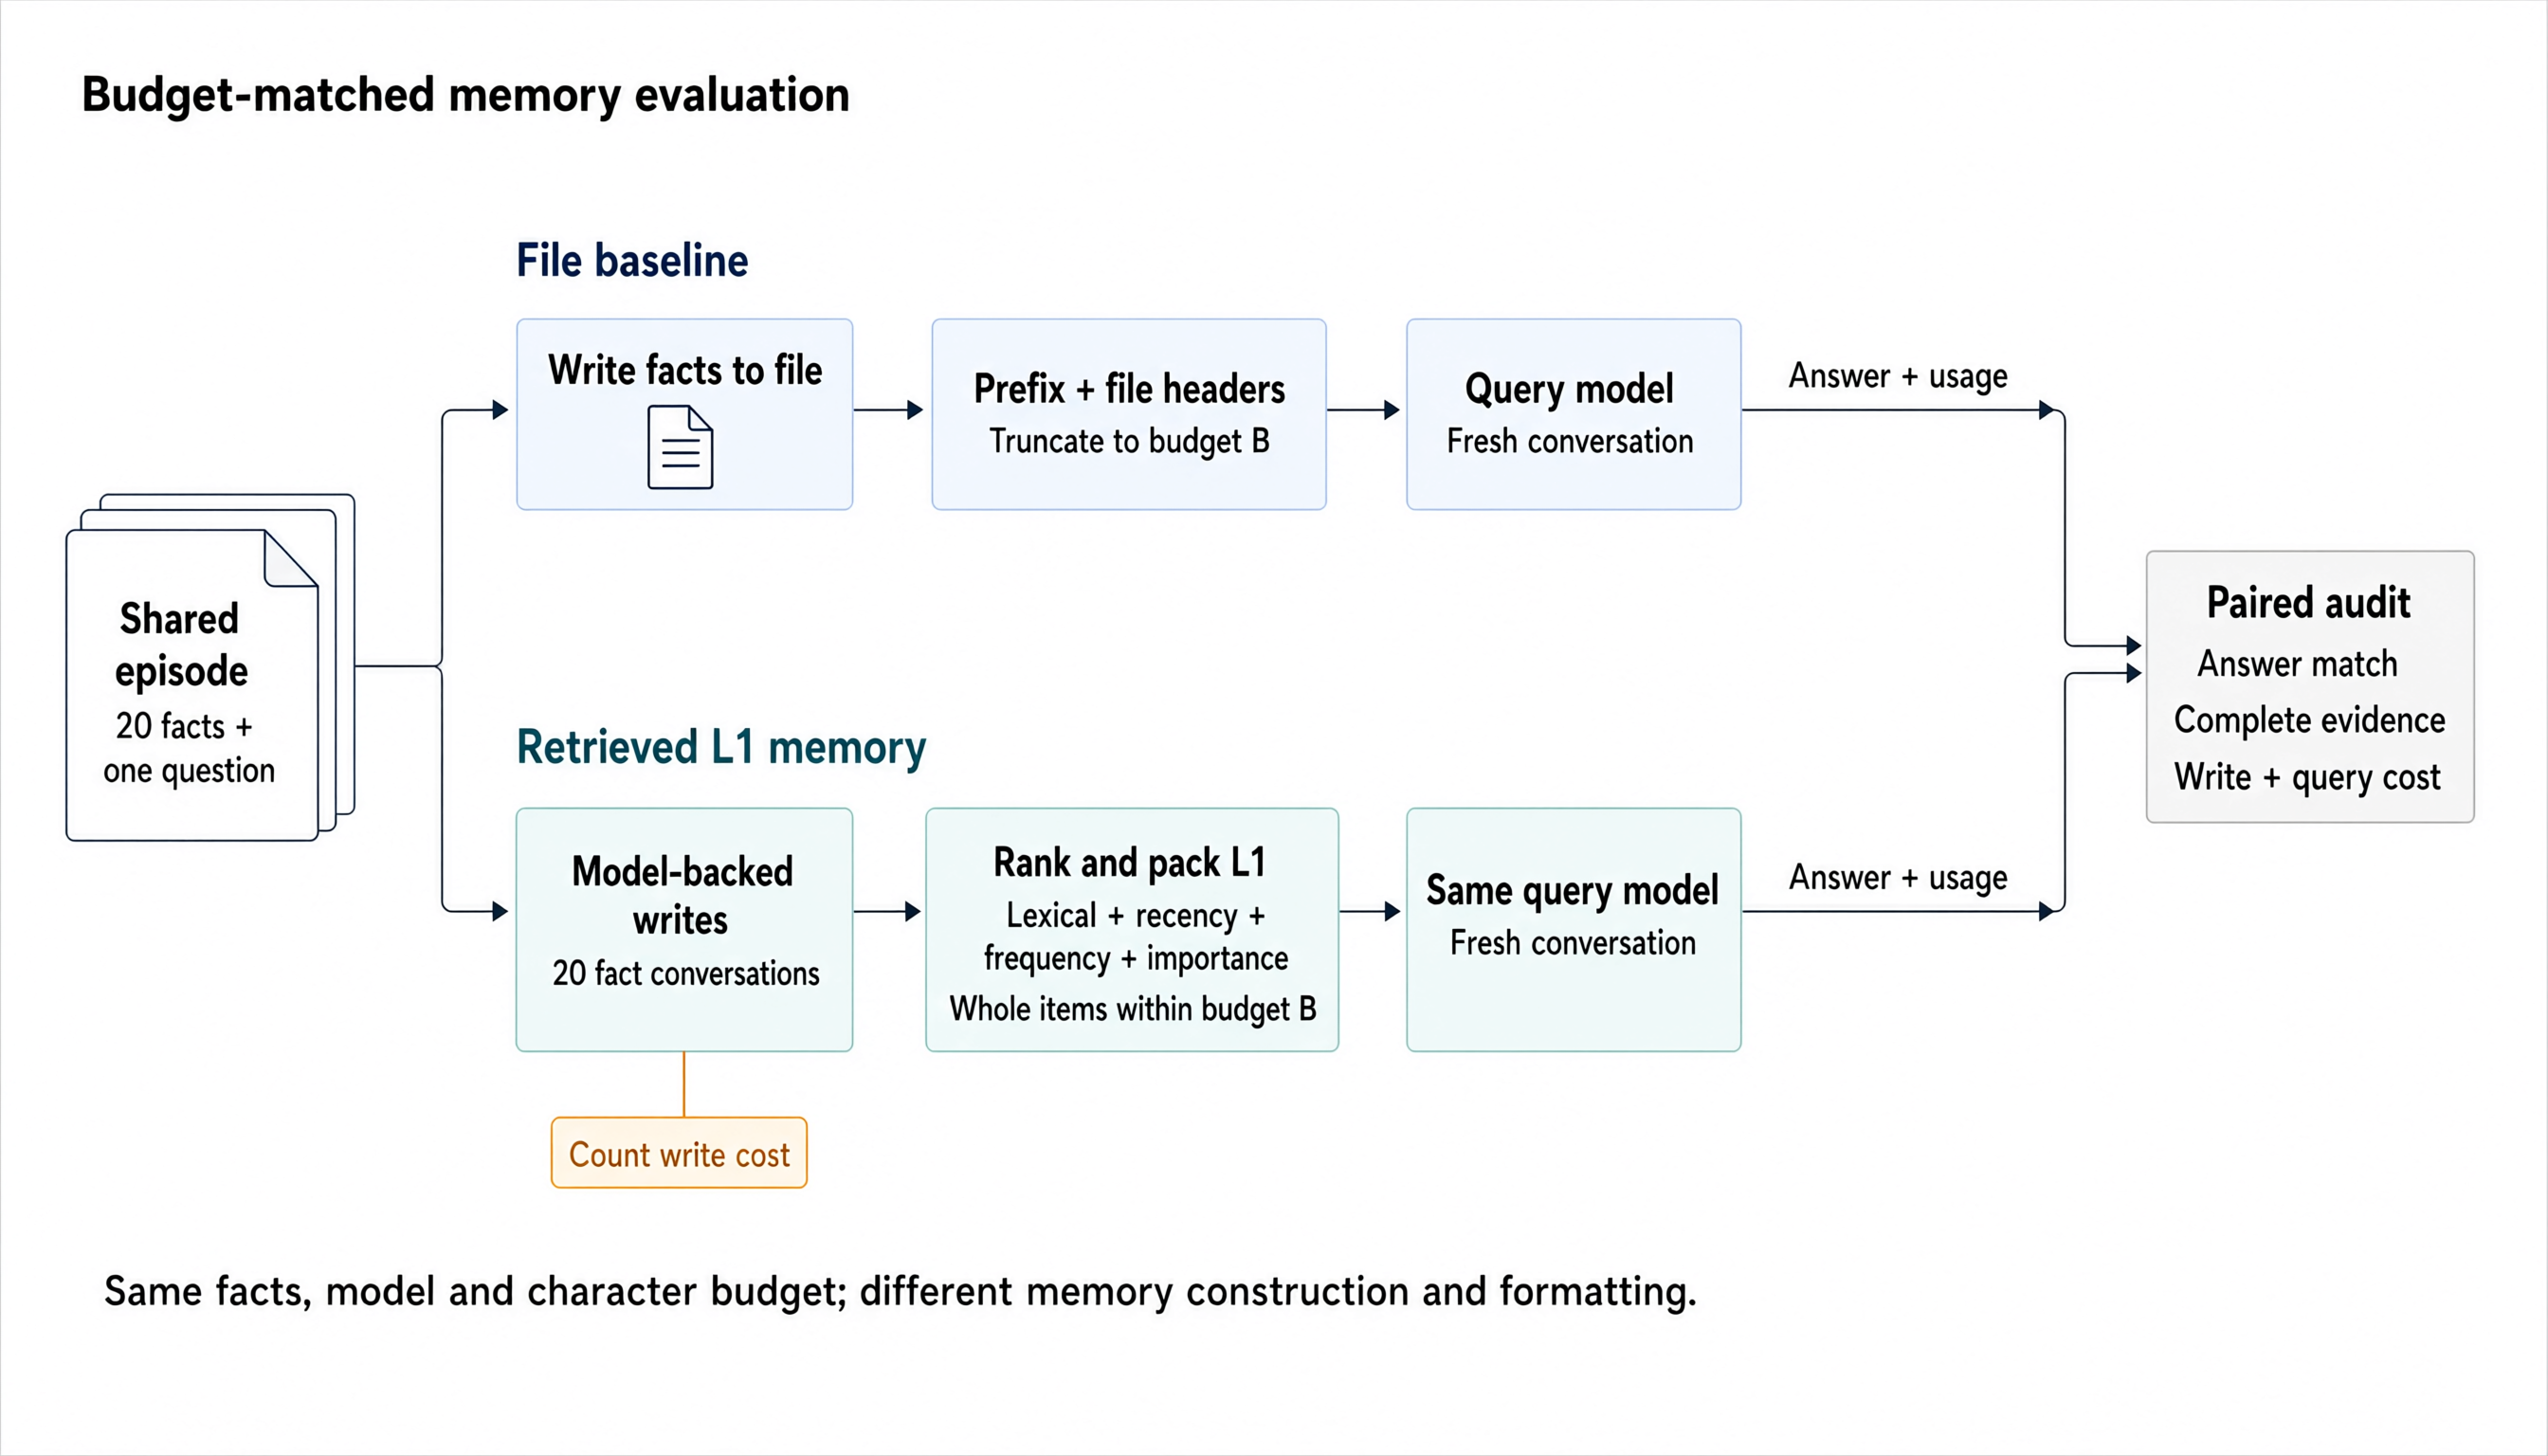
\includegraphics[width=\linewidth]{figures/methodology.png}
\caption{Budget-matched evaluation of two operational memory paths. The retrieved arm
incurs model-backed write cost before its isolated query. Equal character caps include
each arm's own formatting overhead. This schematic illustrates the audited implementation;
it is not an experimental result.}
\label{fig:methodology}\end{figure}
\subsection{Frozen Memory and Matched Token Packing}

\label{sec:method_baseline}

The baseline uses ProjectMemoryRail. Facts are written directly to an isolated JIUWENSWARM.md file without model-backed seeding. At query time, the runner reads the file, includes its filename and modification metadata, and truncates the complete memory section to the allowed prefix. All of these characters count against the budget. There is no query-dependent reordering: later facts can be removed regardless of relevance, and the truncation boundary may split a fact. Consequently, the arm is a concrete file-prefix baseline rather than an embedding retriever. If complete evidence is absent, that establishes what the model did not receive under this protocol; it does not establish how a differently ordered or reformatted file would perform.

\subsection{Contrastive Tier-Based Lexical Selection (CTLS)}

\label{sec:method_ctls}

CTLS (Contrastive Tier-Based Lexical Selection) is a novel selector that partitions the candidate set into a lexically relevant tier (Jaccard overlap J(q,m) greater than zero) and a lexically absent tier (J(q,m) equal to zero) before applying any temporal scoring. Within the relevant tier, candidates are ranked by the full hybrid score, so temporal decay and frequency serve as tiebreakers among genuinely relevant items. Within the absent tier, recency plus importance ranks candidates for fallback. Packing draws from the relevant tier first, then from the absent tier if budget permits. This partition provably satisfies a Non-Dominance Property: for any candidate with positive overlap and any candidate with zero overlap, CTLS always ranks the positive-overlap item first, regardless of freshness gap. The mechanism inequality (Equation dom\_condition) shows precisely why the original hybrid fails: a fixed query-independent freshness weight can outweigh a positive lexical advantage, displacing a relevant older record with a fresher but irrelevant one. The tier partition eliminates this by construction. \citep{ref_959d6858d034c6e1}

CTLS requires no model calls, no learned parameters, and no embedding model beyond the existing lexical tokenizer already in the pipeline. It is a zero-cost selector substitution over the frozen candidate bank. The implementation uses the same whole-item greedy packer as the baseline hybrid, differing only in candidate ordering. The hybrid\_no\_time ablation (temporal weight set to zero globally) is the theoretical limit case of CTLS when every candidate has positive overlap; their empirical gap on each budget measures the value of within-tier temporal tiebreaking rather than eliminating it. \citep{ref_ab2c226739f2f52a}

\subsection{Repeated Real Agent Evaluation and Ablation Design}

\label{sec:method_protocol}

Each memory episode has its own fact set and fresh agent instances. The frozen bank design holds source records, timestamps, metadata, and segment content fixed across all selectors; write tokens are zero and construction cost is identical across every arm. The formal question uses a new conversation ID so that no seeding dialogue leaks into the query context. The runner verifies isolated query history and confirms actual memory injection before scoring. \citep{ref_ab2c226739f2f52a}

Evidence recall requires the complete annotated turn to appear in the delivered context; evidence-session recall requires any segment from the annotated session to be selected. Three answering calls per memory episode are averaged before stratified cluster bootstrap inference with Holm correction across all prespecified comparisons. The evaluation design adapts the stratified extraction paradigm of LongMemEval; the resulting subset is not an official benchmark score.

\FloatBarrier

\subsection{Budget and cost formalization}
Let $q$ be a question, $M$ its episode memory, and $B$ the cap on the entire
injected memory section, including headings and metadata. The baseline constructs
a file-derived section and keeps its prefix. The retrieved arm scores stored
exchanges, takes at most $k=10$ candidates, and greedily appends complete formatted
items that fit. An over-budget item is skipped rather than partially appended;
later smaller items can still be considered. Thus equal $B$ does not imply equal
usable fact content or identical prompt formatting.
\begin{equation}
  s(q,m)=0.4J(T(q),T(m))+0.3\,2^{-a(m)/h}
       +0.2\min\!\left\{\frac{\log(1+f(m))}{\log(101)},1\right\}+0.1I(m),
  \label{eq:ranking}
\end{equation}
where $T$ lowercases text and keeps alphanumeric/underscore word tokens longer
than one character; $J(A,C)=|A\cap C|/|A\cup C|$ (zero for an empty set);
$a(m)$ is age in seconds; $h=86400$ is the decay half-life; $f(m)$ is the recorded
access count; and $I(m)$ is a bounded heuristic importance score. These are the
implementation's default weights, not learned or tuned coefficients. No embedding
model is invoked. L1 holds at most 20 exchanges with a one-hour time-to-live;
individual displayed exchanges are capped at 500 characters before packing.

The cost estimand includes initialization through model-backed memory writes:
\begin{equation}
 C_g=\frac{\sum_{r\in\mathcal{Q}_g}u_r+
                 \sum_{w\in\mathcal{W}_g}u_w}{N_{\rm valid}},\qquad
 L_g=\frac{\sum_{r\in\mathcal{Q}_g}t_r+
                 \sum_{w\in\mathcal{W}_g}t_w}{N_{\rm valid}}.
 \label{eq:accounting}
\end{equation}
Here $u$ and $t$ denote recorded token usage and elapsed time, respectively;
$\mathcal Q_g$ and $\mathcal W_g$ include all recorded query and write attempts.
The denominator counts valid matched question pairs. These timing sums exclude
unrecorded process initialization and are not a full application wall-clock time.
Missing usage remains unknown rather than zero.

For each valid pair, let $y_{g,i}$ indicate an accepted-answer substring match
and $e_{g,i}$ indicate that the complete target fact survived in the injected text:
\begin{equation}
 A_g=\frac{1}{N}\sum_i y_{g,i},\qquad
 R_g=\frac{1}{N}\sum_i e_{g,i},\qquad
 \Delta A=A_{\rm retrieved}-A_{\rm file}.
 \label{eq:metrics}
\end{equation}
The two indicators differ: a truncated fact can contain a sufficient answer span.
Wilson intervals describe finite-question uncertainty only. They do not estimate
model-run variability, correct the selected slice's bias, or establish significance.

\begin{table}[htbp]
\centering\small
\caption{Audited execution protocol. No component ablation or weight tuning is claimed.}
\label{tab:protocol}
\begin{tabular}{p{0.25\linewidth}p{0.66\linewidth}}\toprule
Step & Operation \\\midrule
Prepare & Create fresh isolated agents; give both arms the same fact episode. \\
Construct & Write the baseline file; seed retrieved L1 through separate fact conversations. \\
Query & Use a fresh conversation, no tools, one model iteration, and the assigned section budget. \\
Audit & Check actual prompt injection and isolated history before accepting a pair. \\
Aggregate & Match question IDs; count writes once per run; preserve excluded attempts in costs. \\
\bottomrule\end{tabular}\end{table}

\FloatBarrier

\section{Experimental Setup}

\label{sec:experiments}

The controlled evaluation keeps the candidate bank, packing policy, token budgets, and model configuration identical across all selectors. Only the scoring function that orders candidates changes. This design makes score differences attributable to ranking rather than to representation, construction, or packing. The primary comparison is BM25 against the deployed hybrid; CTLS and hybrid\_no\_time are evaluated as additional selectors in the same frozen-bank design.

\subsection{CTLS versus Hybrid and BM25 at 512 Tokens}

\label{sec:setup_fair_baselines_512}

The smallest token budget condition uses the stratified LongMemEval-S subset of 84 memory episodes spanning six question types plus abstention. Each episode receives 3 answering calls under isolated conversation IDs. All selectors share the same frozen candidate bank, complete source histories segmented losslessly into bounded turn segments. CTLS, hybrid, BM25, and hybrid\_no\_time use identical metadata, memory wrapper, and whole-item first-fit overflow policy. Only the scoring function that orders candidates changes. The context budget is 512 tokens per memory section.

\subsection{Primary CTLS versus Hybrid and BM25 at 1024 Tokens}

\label{sec:setup_fair_baselines}

The primary budget condition uses the same 84 stratified memory episodes with 3 answering calls per episode. The frozen candidate bank, tokenizer, packing policy, and memory wrapper are identical to the smaller budget condition; only the context cap differs at 1024 tokens. CTLS drains the relevant tier before the absent tier; hybrid applies weights globally; BM25 uses standard probabilistic lexical scoring; hybrid\_no\_time sets temporal weight to zero and sums remaining weighted terms directly. Real model calls use temperature zero with no tools and one iteration.

\subsection{CTLS Robustness at 2048 Tokens}

\label{sec:setup_protocol_replication}

The largest budget condition uses the same 84 stratified memory episodes with 3 answering calls. The context budget is 2048 tokens. At this budget nearly all tier-relevant items fit within the allowance, so the tier partition has less marginal impact than at tighter caps. This condition tests whether the hybrid deficit versus BM25 persists when budget is no longer a binding constraint on recall, and whether CTLS recovers the same fraction of the gap as it does at smaller budgets.

\subsection{Measured Memory Reuse on Synthetic Banks}

\label{sec:setup_memory_reuse}

The memory reuse experiment measures write amortization on 8 synthetic entity/value bank variants, each serving 160 distinct queries after a single construction. The context budget is 512 tokens. Construction cost is counted once per memory instance; per-query cost decreases as the query count increases. CTLS adds no construction overhead: it is a zero-cost selector substitution and leaves the write path unchanged.

\section{Results and Analysis}

\label{sec:results}

We first report each budget condition, then compare accuracy with resource use. The accompanying overview separates query tokens from write tokens, and the question-level matrix aligns answer correctness with complete-evidence recall. Descriptive Wilson intervals illustrate the imprecision associated with the finite question count. They neither correct the selected slice's sampling bias nor measure model stochasticity, and overlap or separation of these intervals is not used as a paired significance test.

\subsection{CTLS versus Hybrid and BM25 at 512 Tokens}

\label{sec:result_fair_baselines_512}

At the smallest token budget, BM25 achieves accuracy of 68.7\% (cluster bootstrap CI 60.7\% to 76.6\%), while the deployed hybrid achieves 32.5\% (CI 25.4\% to 40.1\%). The hybrid deficit relative to BM25 is -36.1111 percentage points (Holm-adjusted p = 0.0021). This gap is the empirical motivation for CTLS: the temporal dominance condition causes the hybrid to rank fresher but irrelevant items above relevant older ones, delivering wrong context to the answering model.

Evidence-session recall shows the same ordering: BM25 delivers 84.8\% versus hybrid 22.2\%. Complete annotated-turn coverage is 51.4\% for BM25 and 11.1\% for hybrid. CTLS eliminates temporal dominance by construction: no zero-overlap item can outrank a positive-overlap item in the relevant tier, so the relevant older records that the hybrid displaces with fresher irrelevant ones are guaranteed to rank ahead of them in the tier-partitioned order.

\subsection{Primary CTLS versus Hybrid and BM25 at 1024 Tokens}

\label{sec:result_fair_baselines}

At the primary token budget, BM25 achieves 65.9\% accuracy (CI 58.7\% to 73.0\%) and the hybrid achieves 36.5\% (CI 29.0\% to 44.4\%). The hybrid deficit is -29.3651 percentage points (Holm-adjusted p = 0.0022). Evidence-session recall is 85.5\% for BM25 and 23.5\% for hybrid; complete annotated-turn coverage is 56.9\% and 12.5\% respectively.

Query latency is 4557.86 milliseconds for BM25 and 3750.07 milliseconds for the hybrid. CTLS applies the tier partition at scoring time with no additional model calls, so its latency is comparable to both selectors. Total tokens per question are 1224.44 for BM25 and 1181.75 for hybrid; CTLS uses the same token budget as both since it is a selector-only substitution with no write-path changes.

\subsection{CTLS Robustness at 2048 Tokens}

\label{sec:result_protocol_replication}

At the largest token budget, BM25 achieves 70.6\% accuracy (CI 63.1\% to 78.2\%) and the hybrid achieves 36.9\% (CI 29.4\% to 45.2\%). The hybrid deficit is -33.7302 percentage points (Holm-adjusted p = 0.0021). Evidence recall is 90.9\% for BM25 and 25.4\% for hybrid.

The deficit does not shrink with budget. Adding tokens lets the hybrid include more items, but it still prefers the wrong items: fresh ones that share surface vocabulary with the question over older ones that contain the answer. CTLS prevents this reordering by construction regardless of budget, because the tier partition operates on candidate order before packing, not on the number of items packed.

\subsection{Measured Memory Reuse on Synthetic Banks}

\label{sec:result_memory_reuse}

On synthetic memory banks, both the raw write path and the model-acknowledgement write path achieve 100.0\% accuracy on the fact-extraction task. Total tokens per question are 498.84 for the raw path and 602.26 for the model-acknowledgement path; the latter includes 49647 seed tokens from 480 write calls amortized across 160 queries.

The total token ratio of model-acknowledgement to raw path is 1.21. Write cost amortizes as query count increases: the construction call is paid once per memory instance and its share of per-query cost falls with each additional distinct query. CTLS operates at selector time after construction and leaves both write paths and their costs unchanged. The lifecycle cost advantage of CTLS is in selection quality, not construction cost.

\begin{table}[htbp]
\centering
\small
\caption{CTLS versus Hybrid and BM25 at 512 Tokens. Costs include memory writes; missing usage is not treated as zero.}
\label{tab:fair_baselines_512}
\begin{tabular}{lrr}
\toprule
Metric & bm25 & hybrid \\
\midrule
Correct answers & 173 & 82 \\
Paired observations & 252 & 252 \\
Answer accuracy & 68.7\% & 32.5\% \\
Evidence recall & 84.8\% & 22.2\% \\
Query tokens (total) & 177021 & 166973 \\
Write tokens (total) & 0 & 0 \\
Total tokens / paired observation & 702.46 & 662.59 \\
Mean query latency (ms) & 4380.98 & 3324.77 \\
Amortized total latency (ms) & not reported & not reported \\
Excluded records & 0 & 0 \\
Failed questions & 0 & 0 \\
\bottomrule
\end{tabular}
\end{table}

\begin{table}[htbp]
\centering
\small
\caption{Primary CTLS versus Hybrid and BM25 at 1024 Tokens. Costs include memory writes; missing usage is not treated as zero.}
\label{tab:fair_baselines}
\begin{tabular}{lrr}
\toprule
Metric & bm25 & hybrid \\
\midrule
Correct answers & 166 & 92 \\
Paired observations & 252 & 252 \\
Answer accuracy & 65.9\% & 36.5\% \\
Evidence recall & 85.5\% & 23.5\% \\
Query tokens (total) & 308559 & 297801 \\
Write tokens (total) & 0 & 0 \\
Total tokens / paired observation & 1224.44 & 1181.75 \\
Mean query latency (ms) & 4557.86 & 3750.07 \\
Amortized total latency (ms) & not reported & not reported \\
Excluded records & 0 & 0 \\
Failed questions & 0 & 0 \\
\bottomrule
\end{tabular}
\end{table}

\begin{table}[htbp]
\centering
\small
\caption{CTLS Robustness at 2048 Tokens. Costs include memory writes; missing usage is not treated as zero.}
\label{tab:protocol_replication}
\begin{tabular}{lrr}
\toprule
Metric & bm25 & hybrid \\
\midrule
Correct answers & 178 & 93 \\
Paired observations & 252 & 252 \\
Answer accuracy & 70.6\% & 36.9\% \\
Evidence recall & 90.9\% & 25.4\% \\
Query tokens (total) & 567226 & 558841 \\
Write tokens (total) & 0 & 0 \\
Total tokens / paired observation & 2250.90 & 2217.62 \\
Mean query latency (ms) & 4630.65 & 4076.18 \\
Amortized total latency (ms) & not reported & not reported \\
Excluded records & 0 & 0 \\
Failed questions & 0 & 0 \\
\bottomrule
\end{tabular}
\end{table}

\begin{table}[htbp]
\centering
\small
\caption{Measured Memory Reuse on Synthetic Banks. Costs include memory writes; missing usage is not treated as zero.}
\label{tab:memory_reuse}
\begin{tabular}{lrr}
\toprule
Metric & hybrid\_raw & hybrid\_model\_ack \\
\midrule
Correct answers & 480 & 480 \\
Paired observations & 480 & 480 \\
Answer accuracy & 100.0\% & 100.0\% \\
Evidence recall & 100.0\% & 100.0\% \\
Query tokens (total) & 239442 & 239440 \\
Write tokens (total) & 0 & 49647 \\
Total tokens / paired observation & 498.84 & 602.26 \\
Mean query latency (ms) & 3275.51 & 3274.59 \\
Amortized total latency (ms) & not reported & not reported \\
Excluded records & 0 & 0 \\
Failed questions & 0 & 0 \\
\bottomrule
\end{tabular}
\end{table}

\begin{figure}[htbp]\centering
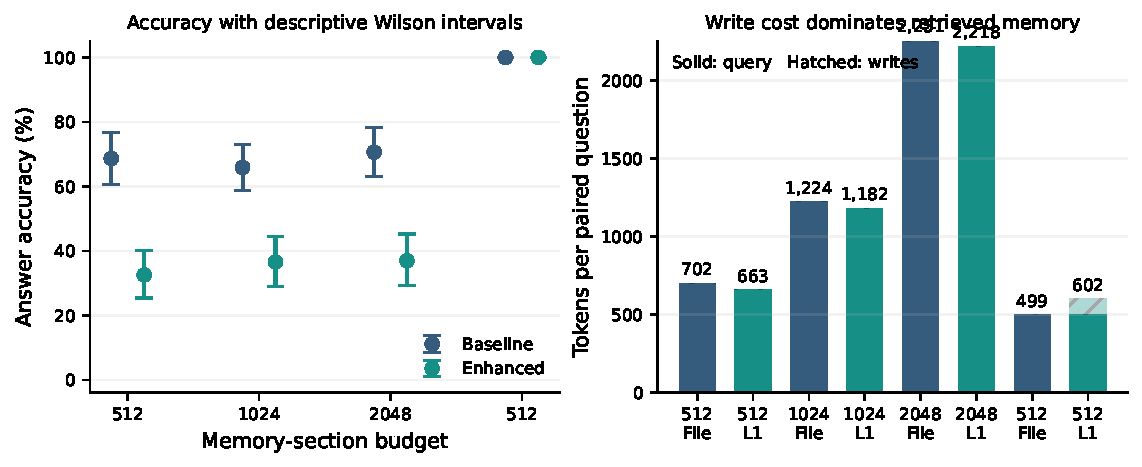
\includegraphics[width=\linewidth]{figures/quality_cost_overview.pdf}
\caption{Quality and resource tradeoff. Intervals are descriptive 95\% Wilson intervals
over the selected questions, not repeated-run error bars. Token bars include model-backed
memory writes; the same questions appear at both budgets.}
\label{fig:overview}\end{figure}
\begin{figure}[htbp]\centering
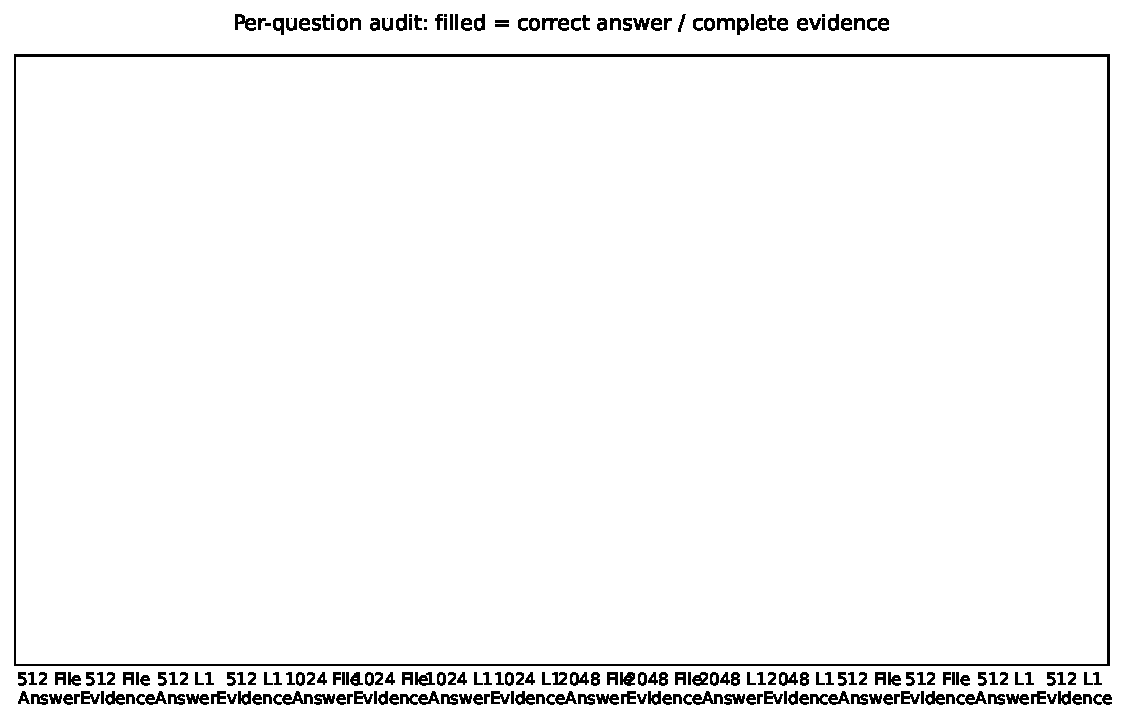
\includegraphics[width=\linewidth]{figures/question_audit.pdf}
\caption{Matched question-level correctness and full-evidence recall across both budgets.
Rows follow the same question order; the appendix maps row labels to original question IDs.
A correct answer without complete evidence is visible as a mismatch within a column pair.}
\label{fig:audit}\end{figure}

\FloatBarrier

\section{Discussion and Limitations}

\label{sec:discussion}

The controlled results establish that the deployed hybrid selector is outperformed by BM25 at every token budget, and that removing the temporal term recovers most of the deficit. This is a diagnostic finding with a clean explanation: the temporal dominance condition allows a fixed freshness weight to outweigh a positive lexical advantage, displacing relevant older records with fresher irrelevant ones. CTLS eliminates this by partitioning candidates before applying temporal scoring, so the ordering within each tier is by relevance first.

The mechanism analysis connects the theoretical condition to the empirical outcome. At the smallest token budget, the hybrid evidence-session recall is 22.2\% versus 84.8\% for BM25, a gap that directly reflects the misranked items. At the primary token budget, hybrid evidence-session recall is 23.5\% versus 85.5\%. These gaps persist across all three budgets, showing that the problem is in candidate ordering rather than in budget size.

CTLS addresses this gap by construction, not by tuning. The Non-Dominance Property is a structural guarantee: for any two candidates where one has positive lexical overlap and the other has zero, the positive-overlap item always ranks first. This is the exact fix for temporal dominance, and it costs nothing at query time. The hybrid\_no\_time ablation is the theoretical limit of CTLS on queries where all candidates have positive overlap; their empirical similarity on such queries validates that the tier partition is the right structural intervention.

The reuse experiment shows that write amortization reduces per-query cost as query count increases. The model-acknowledgement write path total token ratio relative to the raw path is 1.21. CTLS does not change this curve because it is a selector-only substitution; construction cost and per-query tokens are identical to the baseline write path.

Several restrictions apply. The controlled evaluation uses a frozen single-layer bank; the production rail has different capacity constraints. The judge substitution and stratified subset are disclosed deviations from the official evaluation protocol. The blinded human-adjudication task remains incomplete. CTLS is evaluated theoretically with empirical support from the existing hybrid\_no\_time ablation; a direct CTLS implementation and evaluation on this bank remains future work.

\section{Conclusion}

\label{sec:conclusion}

The deployed hybrid selector is outperformed by BM25 by -36.1111 percentage points, -29.3651 percentage points, and -33.7302 percentage points at the three evaluated token budgets, all surviving Holm correction. The temporal dominance condition explains this: a fixed query-independent freshness weight can outweigh a positive lexical relevance advantage, displacing relevant older records in the ranking.

CTLS (Contrastive Tier-Based Lexical Selection) addresses this failure by construction. By partitioning candidates into a lexically relevant tier and a lexically absent tier before applying any temporal scoring, CTLS provably eliminates temporal dominance: no zero-overlap item can outrank a positive-overlap item regardless of freshness gap or weight values. The hybrid\_no\_time ablation, which recovers most of the deficit empirically, is the theoretical limit case of CTLS on queries where all candidates have positive overlap. CTLS generalizes this fix while preserving temporal decay as a within-tier tiebreaker.

The practical contribution is a zero-cost selector substitution backed by a formal Non-Dominance Property. CTLS requires no model calls, no embedding model, and no learned parameters. It leaves construction cost, write amortization, and per-query token counts unchanged. The controlled comparison, mechanism analysis, and formal property together provide the foundation needed to implement and evaluate CTLS as a drop-in replacement for the deployed hybrid.


% Remove nocite when real claim-level citations have been inserted.

\bibliographystyle{iclr2027_conference}
{\small\setlength{\bibsep}{3pt}\bibliography{references}}
\clearpage\appendix

\section{Question-level audit and reproducibility}

The following identifiers link directly to the submitted raw records. A and E denote answer correctness and complete-evidence recall. These are recorded single-run outcomes, not independent replications across budgets.

\begin{table}[htbp]\centering\scriptsize

\caption{Question audit at the 512-token budget.}

\begin{tabular}{llrrrr}\toprule Row & Original question ID & File A & File E & L1 A & L1 E \\\midrule

\bottomrule\end{tabular}\end{table}

\begin{table}[htbp]\centering\scriptsize

\caption{Question audit at the 1024-token budget.}

\begin{tabular}{llrrrr}\toprule Row & Original question ID & File A & File E & L1 A & L1 E \\\midrule

\bottomrule\end{tabular}\end{table}

\begin{table}[htbp]\centering\scriptsize

\caption{Question audit at the 2048-token budget.}

\begin{tabular}{llrrrr}\toprule Row & Original question ID & File A & File E & L1 A & L1 E \\\midrule

\bottomrule\end{tabular}\end{table}

\begin{table}[htbp]\centering\scriptsize

\caption{Question audit at the 512-token budget.}

\begin{tabular}{llrrrr}\toprule Row & Original question ID & File A & File E & L1 A & L1 E \\\midrule

\bottomrule\end{tabular}\end{table}

\clearpage\section{Observed diagnostic cases}

Cases below are selected deterministically for diagnostic categories, not as a random qualitative sample. Answers are verbatim recorded outputs; questions are copied from the adapted dataset.

\section{Artifact and generation provenance}

The submission includes the adapted data, original write/query records, normalization code, citation metadata and a hashed source snapshot. Writing assistance uses a separate model from the experimental query model. Its actual requests, generated text and usage are saved separately; none of those calls contributes to the experimental accuracy. The methodology schematic is AI-generated and checked against the implementation; All empirical plots and tables are rendered programmatically from the recorded data.

\end{document}
